\documentclass[12pt]{article}
\usepackage[margin=1in]{geometry}
\usepackage{amsmath,amssymb,amsthm}
\usepackage{graphicx}
\usepackage{hyperref}
\usepackage{xcolor}
\newlength\tindent
\setlength{\parindent}{0pt}
\setlength{\tindent}{\parindent}
\renewcommand{\indent}{\hspace*{\tindent}}


\usepackage{subcaption}

\title{Phase 03}
\author{Tamzeed Elahi}
\date{\today}



\begin{document}
\maketitle


Code for this project can be found \href{https://github.com/tamzeed-toha/Nonlinear_and_Data_Driven_Estimation/blob/main/project/phase_03.ipynb}{\textcolor{blue}{here}}.

\section*{Project Description}
The problem I am interested for the class project is a system identification problem for a 2D quadrotor system. In the context of this course, the observability of this system will be evaluated; especially for estimating the input matrix which is unknown. 
\begin{align*}
    \dot{x} &= Ax + Bu + w \\
    y &= Cx + v
\end{align*} 
Here, the B matrix is unknown. \\\\
Ultimately, we would be able to estimate the B matrix using the observability matrix and consider the feasibility of a quadrotor system with additional controls (sliding/tilting) like \cite{Nemati2014}. 

\section*{Abstract}



\section*{Introduction}



\section*{Analytical model of quadrotor system}
\begin{figure}[h!]
    \begin{subfigure}[t]{0.5\textwidth}
        \centering
        \includegraphics[width=5cm]{figures/model_diagram.png}
        \caption{Quadrotor system \cite{model_diagram}}
        \label{fig:01}
    \end{subfigure}
    \hfill
    \begin{subfigure}[t]{0.5\textwidth}
        \centering
        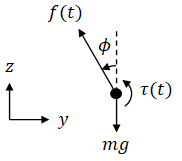
\includegraphics[width=5cm]{figures/free_body_diagram.png}
        \caption{Free body diagram \cite{model_diagram}}
        \label{fig:02}
    \end{subfigure}
\end{figure}
% \includegraphics[width=5cm]{model_diagram.png}

The state space model of a quadrotor system can be found in various literature\cite{K2019}\cite{Schreier2012}. For the class project, I will be using a simplified 2D model (only the y and z coordinates). The dynamic equation of the system can be estimated using Newton's second law of motion.
\begin{align*}
    \ddot{y} &= -\frac{1}{m}u_1(t) \sin{\phi} \\
    \ddot{z} &= -g + \frac{1}{m}u_1(t) \cos{\phi} \\ 
    \ddot{\phi} &= \frac{1}{I_{xx}}u_2(t) \\
\end{align*}
I assumed only two inputs (force and torque) are present in the system. Their relation with the states are nonlinear though it can be linearized with $\phi \approx 0$. It would be more interesting if the inputs are not forces and torques but rotor speeds. \\\\
States are: $x = [\dot{\theta}, \theta, \dot{x}, x, \dot{z}, z]^T$ \\
For now the output matrix-$C$ is considered to be an identity matrix. So, the system assumed to have a GPS and IMU sensors for full state estimation.

inputs are:
\begin{align*}
    u_1(t) &= F \\
    u_2(t) &= \tau
\end{align*}
matrices in continuous form:
\begin{align*}
    A &= \begin{bmatrix}
        0 & 1 & 0 & 0 & 0 & 0 \\
        0 & 0 & 0 & 0 & 0 & 0 \\
        0 & 0 & 0 & 1 & 0 & 0 \\
        0 & 0 & 0 & 0 & 0 & 0 \\
        0 & 0 & 0 & 0 & 0 & 1 \\
        0 & 0 & 0 & 0 & 0 & 0
    \end{bmatrix} \\
    B &= \begin{bmatrix}
        0 & 0 \\
        0 & \frac{1}{I_{xx}} \\
        0 & 0 \\
        - \frac{1}{m} \sin{\theta} & 0 \\
        0 & 0 \\
        \frac{1}{m} \cos{\theta} & 0 \\
    \end{bmatrix} \\
\end{align*}


\pagebreak
\section*{Results:}

\subsection*{Linear case:}
The nonlinearity of this system is due to the input matrix. The input matrix is a function of the states. So, the system is nonlinear. If we consider the unknown parameters of input matrix as a part of the state, then our new A matrix would be:

\begin{align*}
    \dot{x} &= \begin{bmatrix}
        0 & 1 & 0 & 0 & 0 & 0 & 0 & 0 & 0 \\
        0 & 0 & 0 & 0 & 0 & 0 & 0 & 0 & 0 \\
        0 & 0 & 0 & 1 & 0 & 0 & 0 & 0 & 0 \\
        0 & 0 & 0 & 0 & 0 & 0 & 0 & 0 & 0 \\
        0 & 0 & 0 & 0 & 0 & 1 & 0 & 0 & 0 \\
        0 & 0 & 0 & 0 & 0 & 0 & 0 & 0 & 0 \\
        0 & 0 & 0 & 0 & 0 & 0 & 0 & 0 & 0 \\
        0 & 0 & 0 & 0 & 0 & 0 & 0 & 0 & 0 \\
        0 & 0 & 0 & 0 & 0 & 0 & 0 & 0 & 0 \\
    \end{bmatrix} \begin{bmatrix}
        \dot{\theta} \\
        \theta \\
        \dot{x} \\
        x \\
        \dot{z} \\
        z \\
        \beta_1 \\
        \beta_2 \\
        \beta_3 \\
    \end{bmatrix} + \begin{bmatrix}
        0 & 0 \\
        0 & \frac{1}{I_{xx}} \\
        0 & 0 \\
        - \frac{1}{m} \sin{\theta} & 0 \\
        0 & 0 \\
        \frac{1}{m} \cos{\theta} & 0 \\
        0 & 0 \\
        0 & 0 \\
        0 & 0 \\
    \end{bmatrix} \begin{bmatrix}
        F \\
        \tau \\
    \end{bmatrix} 
\end{align*}

Our first task would be to estimate the unknown parameters of the input matrix knowing input matrix using an estimator (Kalman filter). As the A matrix is already linear, we have to discretize it first and then apply the Kalman filter. For our problem, lets break down the input matrix into two parts. One part is known and the other part is unknown.


\begin{align*}
    B_{n \times m} &= B^{0}_{n \times k} B^{1}_{k \times m} \\ 
    \text{so,}  \\
    \dot{x} &= Ax + B^{0} B^{1} u \\
    &= Ax + B^{0} u_{B} \\
    y &= Cx 
\end{align*}
where $B^{0}$ is unknown and $B^{1}$ is known. Here, $B^{0}$ is a row vector but it can be a matrix if the inputs are not linearly independent.

Contiuous form of the system:
\begin{align*}
    \dot{x} &= Ax + B^{0} u_{B} \\
    &= \begin{bmatrix}
        0 & 1 & 0 & 0 & 0 & 0 & 0 & 0 & 0 \\
        0 & 0 & 0 & 0 & 0 & 0 & 0 & 0 & 0 \\
        0 & 0 & 0 & 1 & 0 & 0 & 0 & 0 & 0 \\
        0 & 0 & 0 & 0 & 0 & 0 & 0 & 0 & 0 \\
        0 & 0 & 0 & 0 & 0 & 1 & 0 & 0 & 0 \\
        0 & 0 & 0 & 0 & 0 & 0 & 0 & 0 & 0 \\
        0 & 0 & 0 & 0 & 0 & 0 & 0 & 0 & 0 \\
        0 & 0 & 0 & 0 & 0 & 0 & 0 & 0 & 0 \\
        0 & 0 & 0 & 0 & 0 & 0 & 0 & 0 & 0 \\
    \end{bmatrix} \begin{bmatrix}
        \dot{\theta} \\
        \theta \\
        \dot{x} \\
        x \\
        \dot{z} \\
        z \\
        \beta_1 \\
        \beta_2 \\
        \beta_3 \\
    \end{bmatrix} + \begin{bmatrix}
        0 \\ \frac{1}{I_{xx}} \\ 0 \\ -\frac{1}{m} \\ 0 \\ \frac{1}{m} \\  0 \\ 0 \\ 0
        \end{bmatrix}^{T} \begin{bmatrix}
            0 & 0 \\
            0 & 1 \\
            0 & 0 \\
            \sin{\theta} & 0 \\
            0 & 0 \\
            \cos{\theta} & 0 \\
            0 & 0 \\
            0 & 0 \\
            0 & 0 \\
        \end{bmatrix} \begin{bmatrix}
            F \\
            \tau \\
        \end{bmatrix}
\end{align*}
We know, the continuous form of the system can be discretized using the following equation:
\begin{align*}
    A_d &= e^{A \Delta t}  = \phi(\Delta t) \\
    B_d &= (A_d - I) A^{-1} B \\
    C_d &= C
\end{align*}
In this case, A matrix is singular so we can't use the above equation. We can use the following equation to discretize the system:
\begin{align*}
    A_d &= I + A \Delta t + \frac{A^2 \Delta t^2}{2} + \frac{A^3 \Delta t^3}{6} + \ldots \\
    B_d &= \int_{0}^{\Delta t} e^{A \tau} d\tau B \\
    C_d &= C
\end{align*}
The discretized form of the system is:
\begin{align*}
    A_d &= \begin{bmatrix}
        1 & \Delta t & 0 & 0 & 0 & 0 & 0 & 0 & 0 \\
        0 & 1 & 0 & 0 & 0 & 0 & 0 & 0 & 0 \\
        0 & 0 & 1 & \Delta t & 0 & 0 & 0 & 0 & 0 \\
        0 & 0 & 0 & 1 & 0 & 0 & 0 & 0 & 0 \\
        0 & 0 & 0 & 0 & 1 & \Delta t & 0 & 0 & 0 \\
        0 & 0 & 0 & 0 & 0 & 1 & 0 & 0 & 0 \\
        0 & 0 & 0 & 0 & 0 & 0 & 1 & 0 & 0 \\
        0 & 0 & 0 & 0 & 0 & 0 & 0 & 1 & 0 \\
        0 & 0 & 0 & 0 & 0 & 0 & 0 & 0 & 1 \\
    \end{bmatrix} \\
\end{align*}


\color{black}
Estimation of $B_d$ matrix is a bit tricky because of the singularity of the A matrix. I have estimated the B matrix in two methods:
\begin{enumerate}
    \item Using pseudo-inverse (Moore-Penrose inverse) I got a zero matrix.
    \item Using the integral equation, I got a non-zero matrix. For $\Delta t = 0.1$, the B matrix is: $B_d = \begin{bmatrix}   6.25e-01 \\  1.25e+01 \\ -1.00e-02 \\ -2.00e-01 \\ 1.00e-02 \\ 2.00e-01 \\
        0.00e+00 \\  0.00e+00 \\  0.00e+00 \end{bmatrix}$
\end{enumerate}

\color{black}



Now, we divert our attention to the measurement matrix of the system. The observability of the system is dependent on the measurement matrix. We have to design the measurement matrix in such a way that the system is observable. 

\subsubsection*{Observability}
The observability of the system can be evaluated using the observability matrix. The system is observable if the rank of the observability matrix is equal to the number of states. The observability matrix is given by:
\begin{align*}
    O = \begin{bmatrix}
        C \\
        CA \\
        CA^2 \\
        \vdots \\
        CA^{n-1}
    \end{bmatrix}
\end{align*}

\subsection*{Designing a measurement matrix}
Let's consider the measurement matrix as an identity matrix. 
\begin{align*}
    C &= I
\end{align*}
This makes the system observable (rank = 9). We can get by with lower number of sensors. But, as the beta values don't really have a dynamics, they need direct measurement for estimation. At least for the linear case.

The measurement plot is given below:
\begin{figure}[h!]
    \centering
    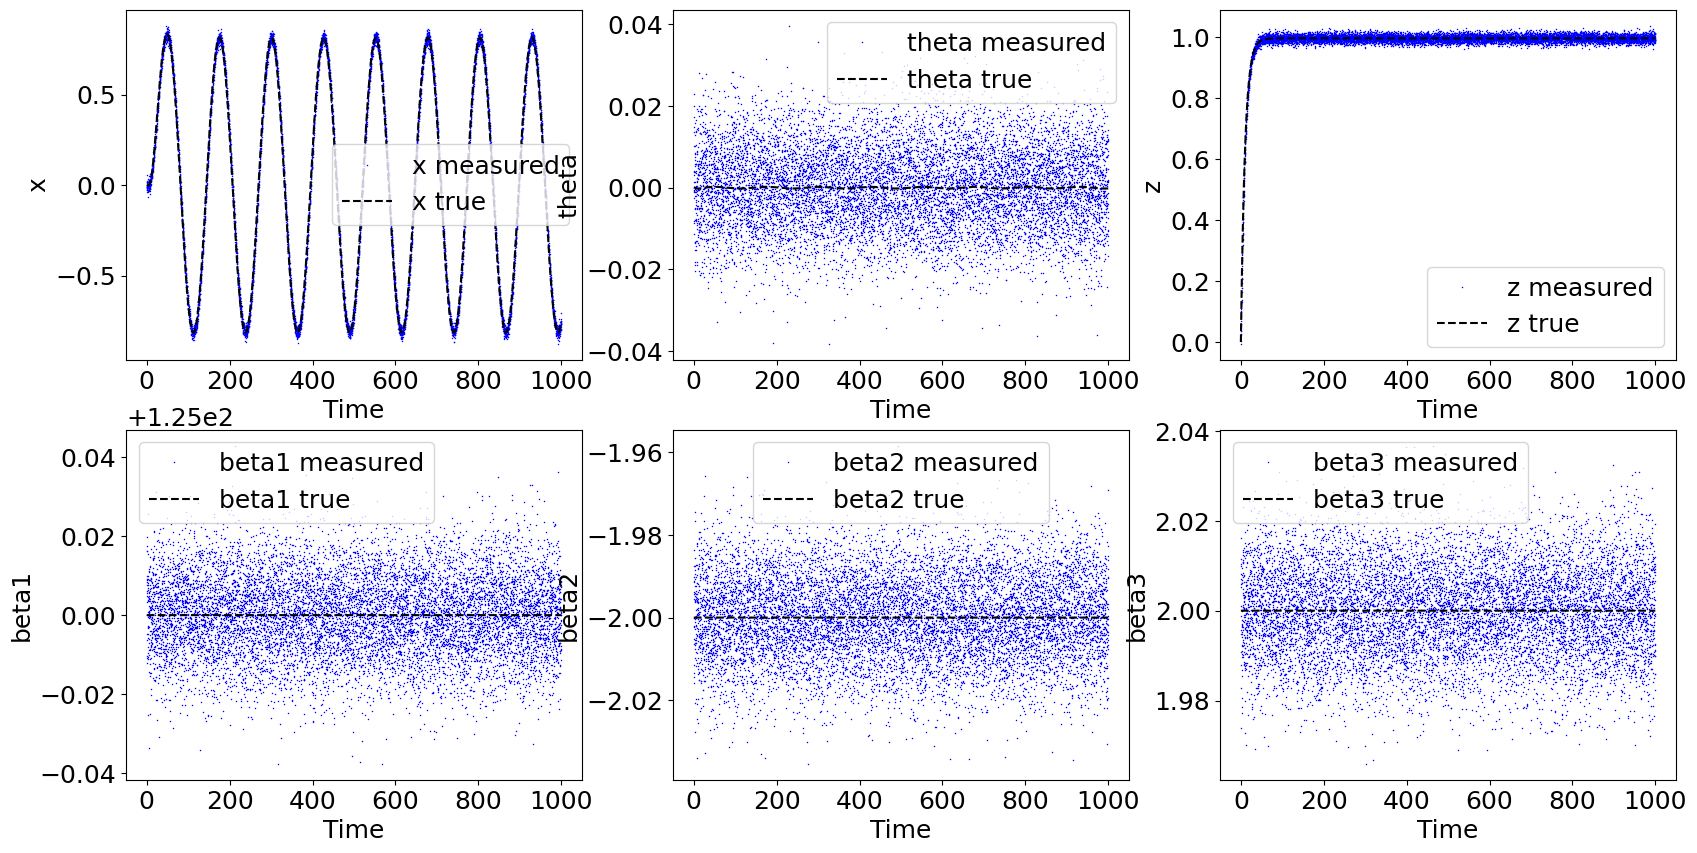
\includegraphics[width=10cm]{figures/phase_02_measurement1.png}
    \caption{Measurement plot}
    \label{fig:03}
\end{figure}
The estimator was able to estimate the states and the unknown parameters of the input matrix. The plot of the estimated states and the true states are given below:
\begin{figure}[h!]
    \centering
    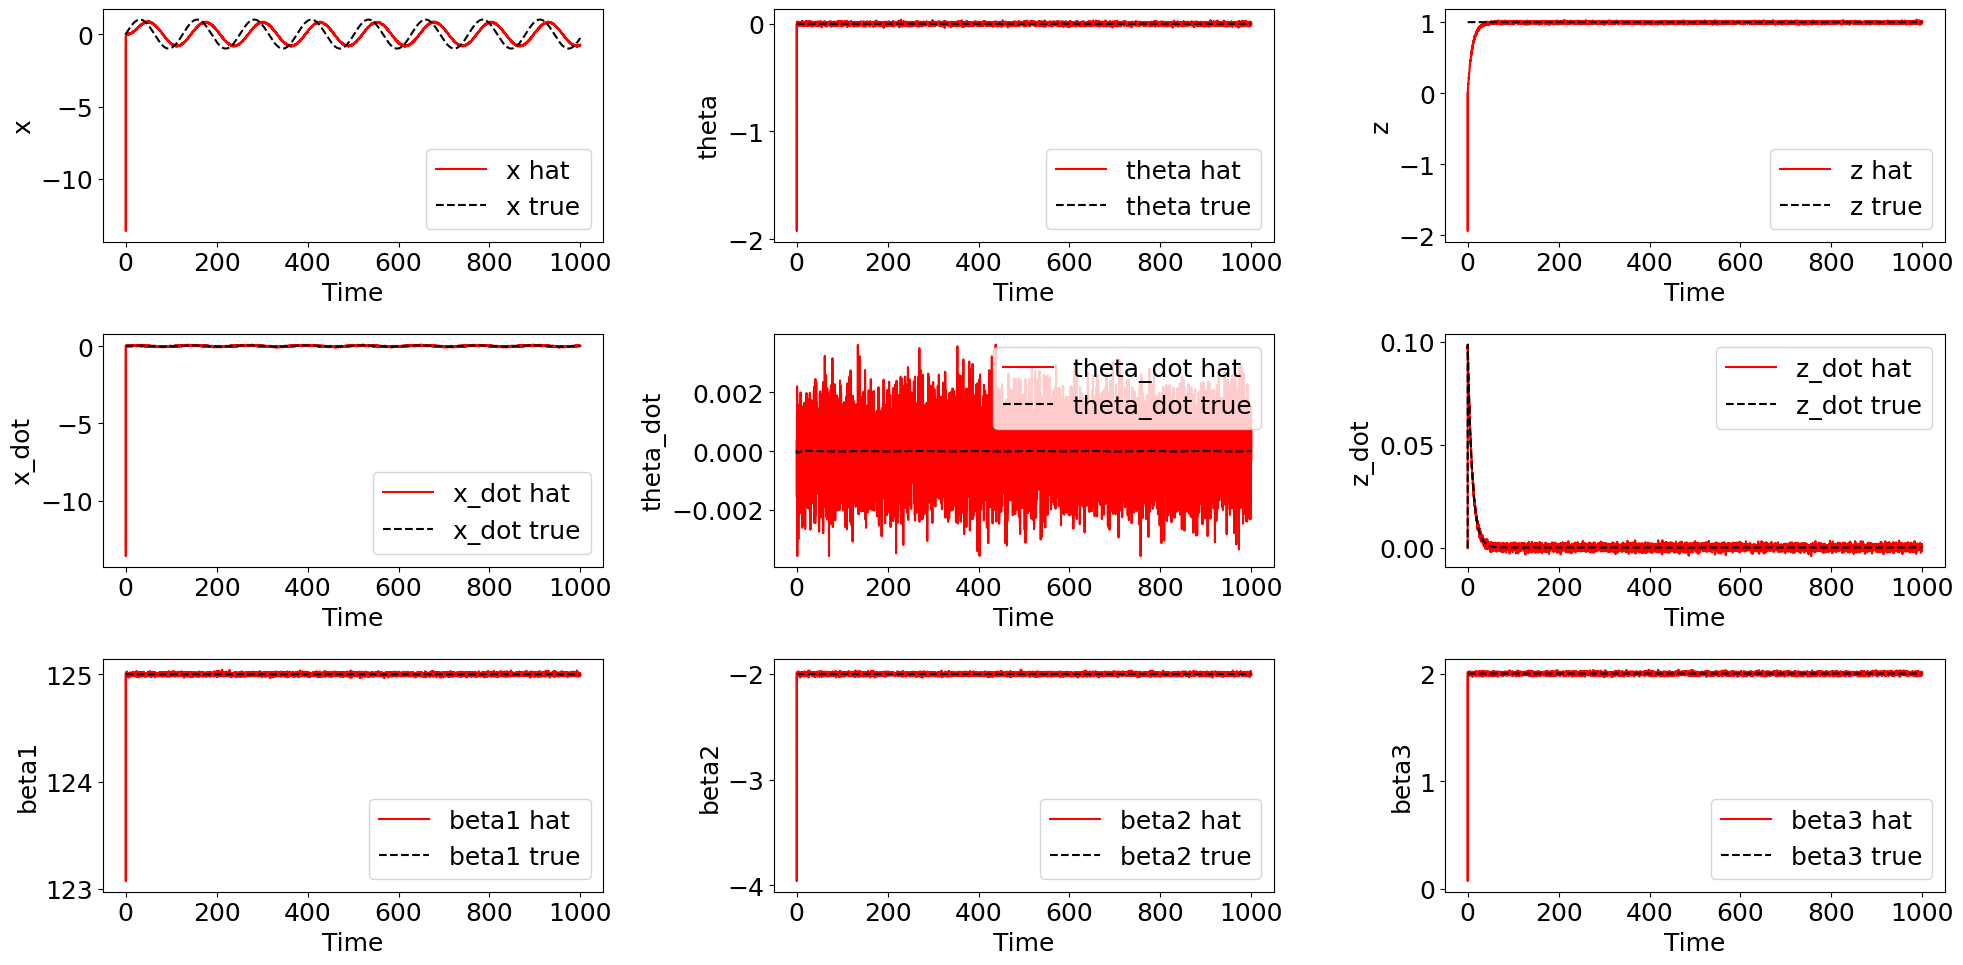
\includegraphics[width=10cm]{figures/phase_02_states1.png}
    \caption{State estimation}
    \label{fig:04}
\end{figure}

\subsection*{Nonlinear case:}
Now lets concentrate our attention to the nonlinear case. The system is nonlinear because it has unknown parameters in the input matrix (and also in the state matrix).  

\section*{Organized dynamic equations:}

States:
\begin{align*}
    \vec{x} &= \begin{bmatrix}
        \colorbox{yellow}{$\dot{\theta}$} \\
        \colorbox{yellow}{$\theta$} \\
        \colorbox{yellow}{$\dot{x}$} \\
        \colorbox{yellow}{$x$} \\
        \colorbox{yellow}{$\dot{z}$} \\
        \colorbox{yellow}{$z$} \\
        \hline
        \colorbox{pink}{$\beta_1$} \\
        \colorbox{pink}{$\beta_2$} \\
        % \colorbox{pink}{$\beta_3$} \\
    \end{bmatrix}
\end{align*}

Dynamic equations:
\begin{align*}
    \dot{\vec{x}} &= \begin{bmatrix}
        \colorbox{yellow}{$\dot{x_1}$} \\
        \colorbox{yellow}{$\dot{x_2}$} \\
        \colorbox{yellow}{$\dot{x_3}$} \\
        \colorbox{yellow}{$\dot{x_4}$} \\
        \colorbox{yellow}{$\dot{x_5}$} \\
        \colorbox{yellow}{$\dot{x_6}$} \\
        \hline
        \colorbox{pink}{$\dot{x_7}$} \\
        \colorbox{pink}{$\dot{x_8}$} \\
        % \colorbox{pink}{$\dot{x_9}$} \\
    \end{bmatrix} = \begin{bmatrix}
        1/I_{xx} \colorbox{green}{$u_2$} \\ 
        \colorbox{yellow}{$x_1$} \\
        1/m \colorbox{green}{$u_1$} \sin{\colorbox{yellow}{$x_2$}} \\
        \colorbox{yellow}{$x_3$} \\
        -g + 1/m \colorbox{green}{$u_1$} \cos{\colorbox{yellow}{$x_2$}} \\
        \colorbox{yellow}{$x_6$} \\
        \hline
        0 \\
        0 \\
        % 0 \\
    \end{bmatrix} = \begin{bmatrix}
        \colorbox{pink}{$x_7$} \colorbox{green}{$u_2$} \\
        \colorbox{yellow}{$x_1$} \\
        \colorbox{pink}{$x_8$} \colorbox{green}{$u_1$} \sin{\colorbox{yellow}{$x_2$}} \\
        \colorbox{yellow}{$x_3$} \\
        -\colorbox{cyan}{g} + \colorbox{pink}{$x_8$} \colorbox{green}{$u_1$} \cos{\colorbox{yellow}{$x_2$}} \\
        \colorbox{yellow}{$x_6$} \\
        \hline
        0 \\
        0 \\
        % 0 \\
    \end{bmatrix} \\
    &= \begin{bmatrix}
        0 \\
        \colorbox{yellow}{$x_1$} \\
        0 \\
        \colorbox{yellow}{$x_3$} \\
        -\colorbox{cyan}{g} \\
        \colorbox{yellow}{$x_6$} \\
        \hline
        0 \\
        0 \\
        % 0 \\
        \end{bmatrix} + \begin{bmatrix}
        0 \\
        0 \\
        \colorbox{pink}{$x_8$} \sin{\colorbox{yellow}{$x_2$}} \\
        0 \\
        \colorbox{pink}{$x_8$} \cos{\colorbox{yellow}{$x_2$}} \\
        0 \\
        \hline
        0 \\
        0 \\
        % 0 \\
    \end{bmatrix} \colorbox{green}{$u_1$} + \begin{bmatrix}
        \colorbox{pink}{$x_7$} \\
        0 \\
        0 \\
        0 \\
        0 \\
        0 \\
        \hline
        0 \\
        0 \\
        % 0 \\
    \end{bmatrix} \colorbox{green}{$u_2$} \\    
    % \dot{\vec{x}} &= \begin{bmatrix}
    %     \colorbox{pink}{$\beta_1$} \colorbox{lime}{$u_2$} \\
    %     \colorbox{yellow}{$\dot{\theta}$} \\
    %     \colorbox{pink}{$\beta_2$} \colorbox{lime}{$u_1$} \sin{\colorbox{yellow}{$\theta$}} \\ 
    %     \colorbox{yellow}{$\dot{x}$} \\
    %     -\colorbox{cyan}{g}+\colorbox{pink}{$\beta_3$} \colorbox{lime}{$u_1$} \cos{\colorbox{yellow}{$\theta$}} \\
    %     \colorbox{yellow}{$\dot{z}$} \\
    %     \hline
    %     0 \\
    %     0 \\
    %     0 \\
    % \end{bmatrix} \\
    % &= \begin{bmatrix}
    %         0 \\
    %         \colorbox{yellow}{$\dot{\theta}$} \\
    %         0 \\
    %         \colorbox{yellow}{$\dot{x}$} \\
    %         -\colorbox{cyan}{g} \\
    %         \colorbox{yellow}{$\dot{z}$} \\
    %         \hline
    %         0 \\
    %         0 \\
    %         % 0 \\
    %     \end{bmatrix} +  \begin{bmatrix}
    %         0 \\
    %         0 \\
    %         \colorbox{pink}{$\beta_2$} \sin{\colorbox{yellow}{$\theta$}} \\
    %         0 \\
    %         \colorbox{pink}{$\beta_3$} \cos{\colorbox{yellow}{$\theta$}} \\
    %         0 \\
    %         \hline
    %         0 \\
    %         0 \\
    %         % 0 \\
    %     \end{bmatrix} \colorbox{lime}{$u_1$} +  \begin{bmatrix}
    %         \colorbox{pink}{$\beta_1$} \\
    %         0 \\
    %         0 \\
    %         0 \\
    %         0 \\
    %         0 \\    
    %         \hline        
    %         0 \\
    %         0 \\
    %         % 0 \\
    %     \end{bmatrix} \colorbox{lime}{$u_2$} \\
    &= \begin{bmatrix}
        0 \\
        \colorbox{yellow}{$\dot{\theta}$} \\
        0 \\
        \colorbox{yellow}{$\dot{x}$} \\
        -\colorbox{cyan}{g} \\
        \colorbox{yellow}{$\dot{z}$} \\
        \hline
        0 \\
        0 \\
        % 0 \\
    \end{bmatrix} +  \begin{bmatrix}
        0 \\
        0 \\
        % \colorbox{pink}{$\beta_2$} \\
        \colorbox{pink}{$x_8$} \\
        0 \\
        % \colorbox{pink}{$\beta_3$} \\
        \colorbox{pink}{$x_8$} \\
        0 \\
        \hline
        0 \\
        0 \\
        % 0 \\
    \end{bmatrix} \colorbox{lime}{$\tilde{u}_1$} + \begin{bmatrix}
        % \colorbox{pink}{$\beta_1$} \\
        \colorbox{pink}{$x_7$} \\
        0 \\
        0 \\
        0 \\
        0 \\
        0 \\ 
        \hline
        0 \\
        0 \\
        % 0 \\
    \end{bmatrix} \colorbox{lime}{$u_2$} \\
    &= f_0(\vec{x}) + f_1(\vec{x}) \tilde{u}_1 + f_2(\vec{x}) u_2
\end{align*}

where, 
\begin{align*}
    \tilde{u}_1 &= \begin{bmatrix}
        0 \\
        0 \\
        % \sin{\colorbox{yellow}{$\theta$}} \\
        \sin{\colorbox{yellow}{$x_2$}} \\
        0 \\
        % \cos{\colorbox{yellow}{$\theta$}} \\
        \cos{\colorbox{yellow}{$x_2$}} \\
        0 \\
        \hline
        0 \\
        0 \\
        % 0 \\
    \end{bmatrix} u_1
\end{align*}

known constants: \colorbox{cyan}{$g$} = 9.81 $m/s^2$ \\

Measurement matrix: I have played around with different measurement matrices and trajectories. Observability analysis and state estimation for all those measurements are given below.
\begin{align*}
    h &= \left[\begin{matrix}\dot{\theta}\\\theta\\\dot{x}\\x\\\dot{z}\\z\\\beta_{1}\\\beta_{2}\\\beta_{3}\end{matrix}\right], 
    \left[\begin{matrix}\theta\\x\\z\end{matrix}\right],
    \left[\begin{matrix}\theta\\x\end{matrix}\right], 
    \left[\begin{matrix}\theta x z\end{matrix}\right], 
    \left[\begin{matrix}\theta\\x z\end{matrix}\right],
    \left[\begin{matrix}\theta\\x + z\\z\end{matrix}\right],
    \left[\begin{matrix}\theta + x\\x + z\end{matrix}\right],
    \left[\begin{matrix}\theta + x\\x + z\\\theta + z\end{matrix}\right],
    \left[\begin{matrix}\theta x\\\frac{z}{x}\\\theta + z\end{matrix}\right],
    \left[\begin{matrix}\theta x\\\frac{z}{x}\end{matrix}\right]
\end{align*}

\subsection*{Observability analysis:}
First, we will estimate the observability of the system analytically for different measurement system. We have to estimate G matrix which is the collection of all unique lie-derivatives of the system. 
\begin{align*}
    G &= \left[\begin{matrix}0\\- g\\\theta\\x\\\beta_{3}\\\dot{\theta}\\\beta_{1}\\\beta_{2}\\z\\\dot{x}\\\dot{z}\end{matrix}\right], 
    \left[\begin{matrix}0\\- g\\\theta\\x\\\beta_{3}\\\dot{\theta}\\\beta_{1}\\\beta_{2}\\z\\\dot{x}\\\dot{z}\end{matrix}\right], 
    \left[\begin{matrix}0\\\theta\\x\\\dot{x}\\\dot{\theta}\\\beta_{1}\\\beta_{2}\end{matrix}\right], 
    \left[\begin{matrix}0\\\beta_{1} x z\\\theta x z\\\beta_{2} \theta z + \beta_{3} \theta x\\\dot{\theta} x z + \dot{x} \theta z + \dot{z} \theta x\\\dot{\theta} \left(\dot{x} z + \dot{z} x\right) + \dot{x} \left(\dot{\theta} z + \dot{z} \theta\right) + \dot{z} \left(\dot{\theta} x + \dot{x} \theta\right) - g \theta x\end{matrix}\right],
    \left[\begin{matrix}0\\\dot{x} z + \dot{z} x\\x z\\\theta\\\beta_{2} z + \beta_{3} x\\\dot{\theta}\\2 \dot{x} \dot{z} - g x\\\beta_{1}\end{matrix}\right] \\
    &= ,\left[\begin{matrix}0\\- g\\\theta\\\beta_{3}\\\dot{\theta}\\\beta_{1}\\x + z\\z\\\beta_{2} + \beta_{3}\\\dot{x} + \dot{z}\\\dot{z}\end{matrix}\right],
    \left[\begin{matrix}0\\- g\\\beta_{2} + \beta_{3}\\\beta_{2}\\\theta + x\\\dot{\theta} + \dot{x}\\\dot{x} + \dot{z}\\\beta_{1}\\x + z\end{matrix}\right],
    \left[\begin{matrix}0\\- g\\\dot{\theta} + \dot{z}\\\beta_{3}\\\theta + x\\\beta_{1}\\x + z\\\beta_{2}\\\beta_{2} + \beta_{3}\\\dot{\theta} + \dot{x}\\\dot{x} + \dot{z}\\\theta + z\end{matrix}\right],
    \left[\begin{matrix}0\\- g\\\dot{\theta} x + \dot{x} \theta\\\dot{\theta} + \dot{z}\\\beta_{3}\\2 \dot{\theta} \dot{x}\\- \frac{\dot{x} z}{x^{2}} + \frac{\dot{z}}{x}\\\theta x\\\frac{z}{x}\\- \frac{\beta_{2} z}{x^{2}} + \frac{\beta_{3}}{x}\\\beta_{1}\\- \frac{\dot{x} \dot{z}}{x^{2}} + \dot{x} \left(\frac{2 \dot{x} z}{x^{3}} - \frac{\dot{z}}{x^{2}}\right) - \frac{g}{x}\\\beta_{1} x\\\theta + z\\\beta_{2} \theta\end{matrix}\right],
    \left[\begin{matrix}0\\- \frac{\dot{x} \dot{z}}{x^{2}} + \dot{x} \left(\frac{2 \dot{x} z}{x^{3}} - \frac{\dot{z}}{x^{2}}\right) - \frac{g}{x}\\\dot{\theta} x + \dot{x} \theta\\\beta_{1} x\\2 \dot{\theta} \dot{x}\\\beta_{2} \theta\\- \frac{\dot{x} z}{x^{2}} + \frac{\dot{z}}{x}\\\theta x\\\frac{z}{x}\\- \frac{\beta_{2} z}{x^{2}} + \frac{\beta_{3}}{x}\end{matrix}\right]
\end{align*}
Taking the jacobian on the G matrix, we can estimate the observability matrix of the system. The rank of the observability matrix if it is greater than the number of states, makes the system observable.
I have both analytically and numerically estimated the observability of the system for different measurements, trajectories and state values. They dont seem to be time variant. One interesting observation is that the rank values estimated by the two methods are not the same for all cases (Further investigation is needed).

\begin{figure}[h!]
    \begin{subfigure}[t]{0.5\textwidth}
        \centering
        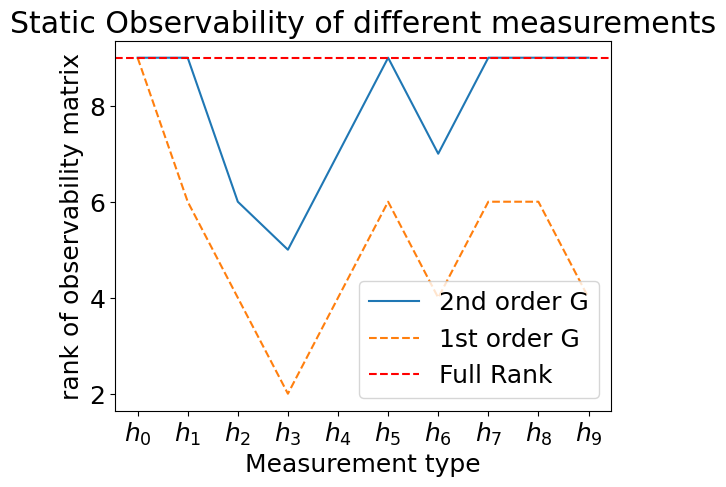
\includegraphics[width=5cm]{figures/phase_03_obswithh.png}
        \caption{Observability of different measurements}
        \label{fig:05}
    \end{subfigure}
    \hfill
    \begin{subfigure}[t]{0.5\textwidth}
        \centering
        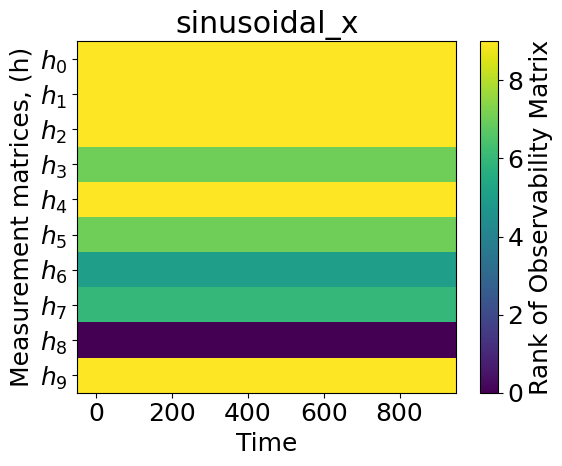
\includegraphics[width=5cm]{figures/phase_03_obswithtime.png}
        \caption{Observability of different measurements with time}
        \label{fig:06}
    \end{subfigure}
\end{figure}
Another approach to estimate the observability of the system is to use the emperical observability method. For $h_0$, which should be the most observable state, the E-ISO results are given below:
\begin{figure}[h!]
    \centering
    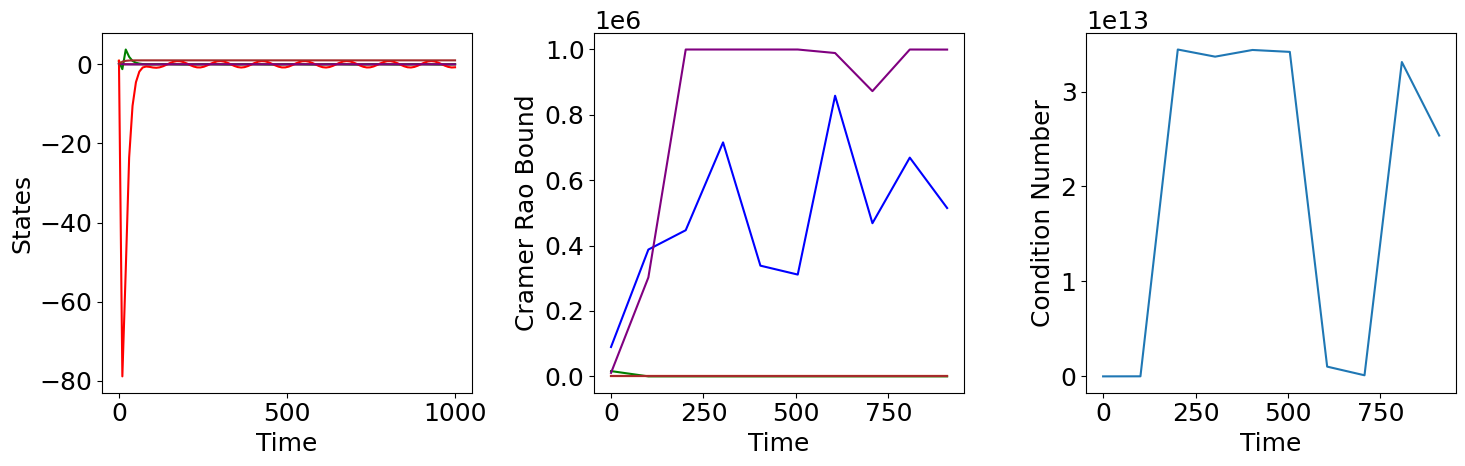
\includegraphics[width=10cm]{figures/phase_03_emperical1.png}
    \caption{Emperical observability of h0}
    \label{fig:07}
\end{figure}
For $h_1$, which is the more realistic measurement matrix, the E-ISO results are given below:
\begin{figure}[h!]
    \centering
    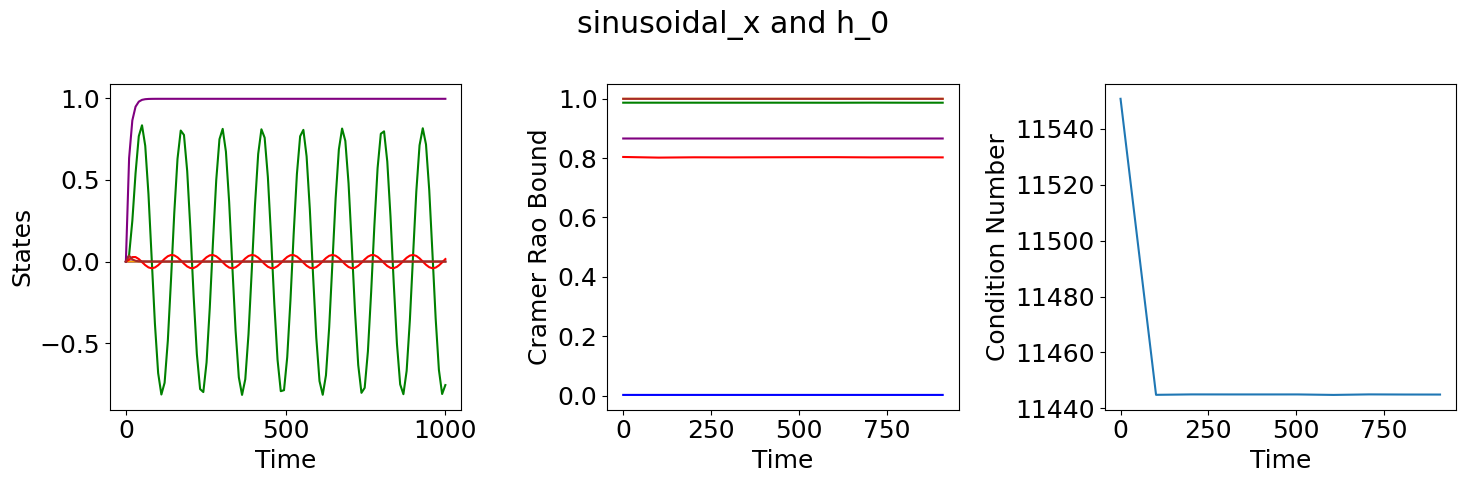
\includegraphics[width=10cm]{figures/phase_03_emperical2.png}
    \caption{Emperical observability of h1}
    \label{fig:08}
\end{figure}
The observability analysis of the model is not yet perfect. The observability values dont oscillate with time. And the Cramer Rao lower bound is also too high in most cases. 


\subsection*{State estimation:}
As my system is non-linear, I am using extended Kalman filter for state estimation. For the same sinusoidal trajectory, output y is:
\begin{figure}[h!]
    \centering
    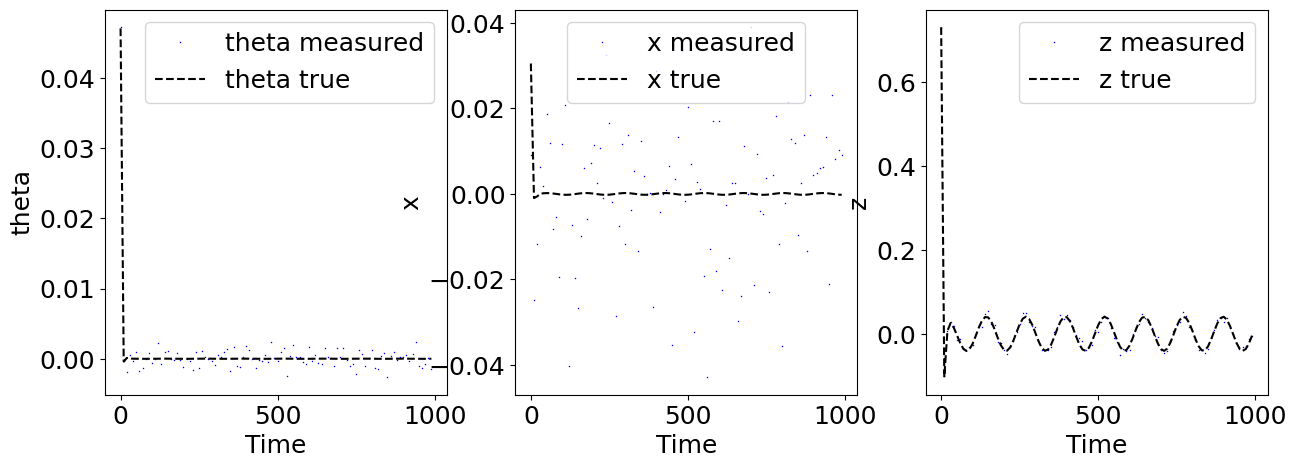
\includegraphics[width=10cm]{figures/phase_03_outputy1.png}
    \caption{state measurements}
    \label{fig:09}
\end{figure}
For this output (y) and different measurement matrices, the state estimation of unknown parameters of the input matrix are given below:

\begin{figure}[h!]
    \begin{subfigure}[t]{\textwidth}
        \centering
        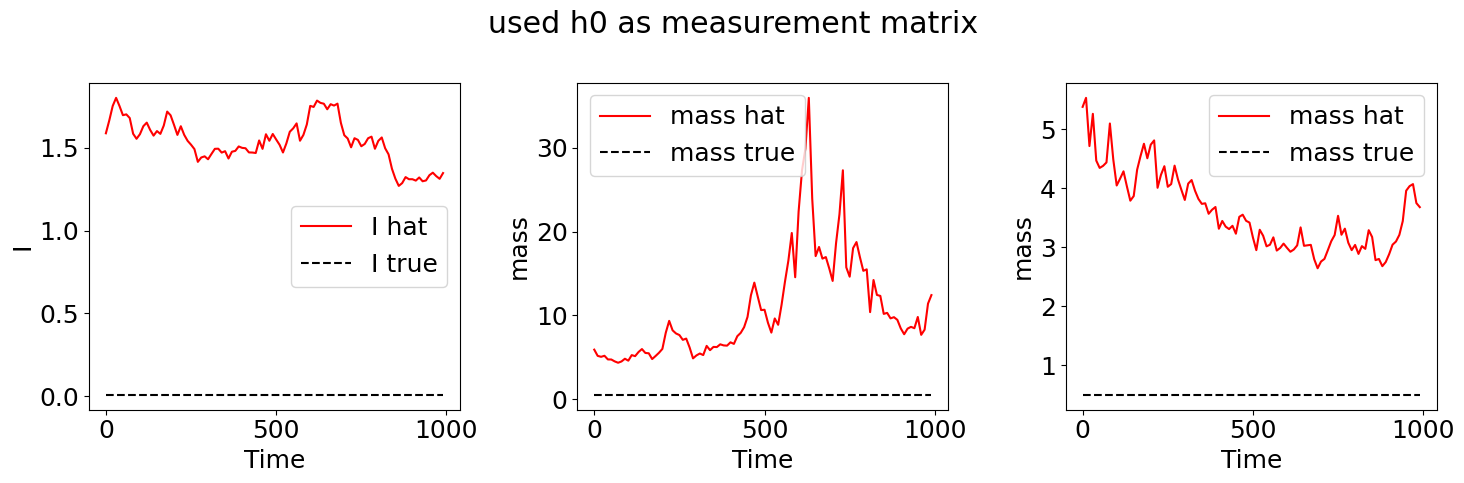
\includegraphics[width=10cm]{figures/phase_03_param1.png}
        \caption{State estimation with h0}
        \label{fig:10}
    \end{subfigure}
    \\
    \begin{subfigure}[t]{\textwidth}
        \centering
        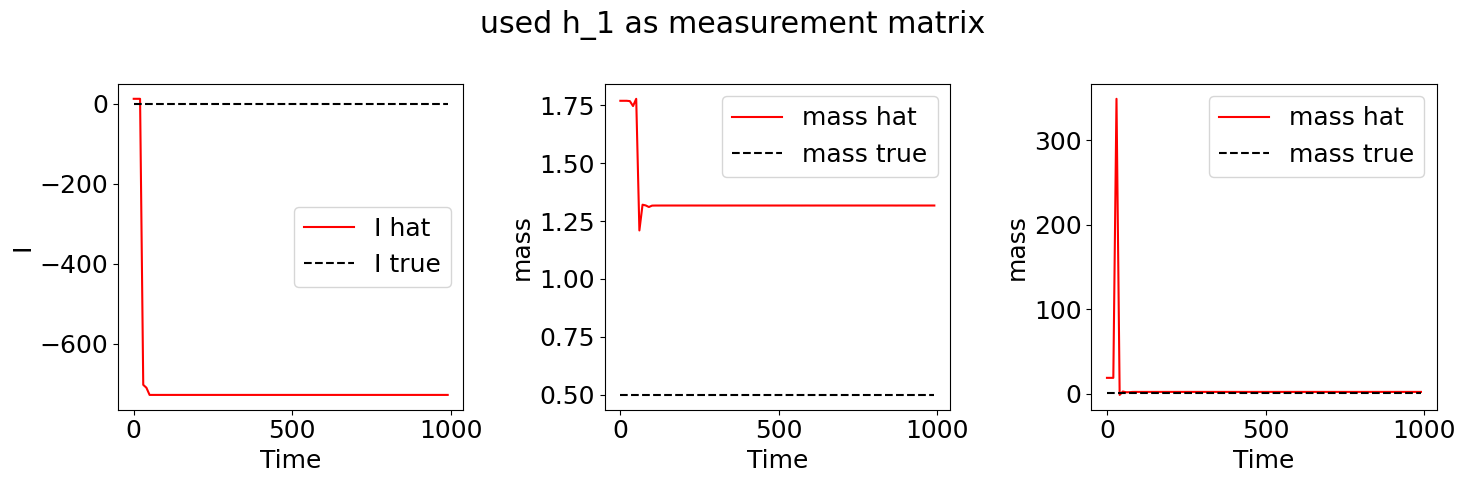
\includegraphics[width=10cm]{figures/phase_03_param2.png}
        \caption{State estimation with h1}
        \label{fig:11}
    \end{subfigure}
\end{figure}

More investigation can be found in the associated code.

\pagebreak
\section*{Conclusion}

\pagebreak
\bibliographystyle{plain}
\bibliography{phase0}









\end{document}